\section{Literature Review and Theoretical Background}
\label{sec: lit_rev}

In this chapter I will provide an overview about influential literature and the theoretical foundations in the fields of volatility forecasting. Moreover, I will elaborate on related work that used textual contents (of corporate filings) in empirical finance and accounting. Finally, a short overview about commonly used techniques in text mining, text classification, and sentiment analysis within the financial framework is provided.

% ----------------------------------------------------------- %

\subsection{Volatility Forecasting}
\label{ssec: lit_rev_vola}

\subsubsection{Simple and Exponentially-Weighted Moving Average}
\label{sssec: lit_rev_vola_ma}

The most basic model to capture time variation in the conditional variance is to let the volatility series follow a very simple $m$-period moving average process.
\begin{align*}
\text{MA(m): }\qquad & r_t = \mu_{t} + e_{t}, \quad e_{t} = \sigma_{t} z_{t},\quad  z_{t} \overset{\text{iid}}{\sim} \mathcal{G}(0,1) \\
& \sigma_t^2 = 1/m \sum_{i=0}^m (r_{t-i-1} - \bar{r})^2, \numberthis 
\end{align*}

where  $r_t$ is the time series of continuously compounded asset returns and $\mu_{t} = \expect{r_t|\mathcal{F}_{t-1}}$ is the conditional mean series\footnote{We call it \emph{conditional} because it depends on the information set available in $t-1$, which we will denote by $\mathcal{F}_{t-1}$. Often, however, we will simplify notation and abbreviate to \enquote{mean series}.}. Very often one assumes $\mu_{t}$ to be constant over time ($ \mu_{t}=\mu $), or even zero ($ \mu_{t}=\mu=0 $)\footnote{This is often an acceptable assumption, especially when the data is sampled from high frequencies (e.g., daily or intra-daily).}. Otherwise, the conditional mean series usually is described by some simple process out of the ARMA family.
Note that in this model the assumption of a zero mean series would imply $\bar{r}=0$, which eases the notational tediousness, as the current variance can be expressed as a simple average of the past $m$ period's squared returns: $\sigma_t^2 = 1/m \sum_{i=0}^m r_{t-i-1}^2 $.

Furthermore, in terms of notation, the series $e_t$ is referred to as \enquote{innovation process}, whilst also \enquote{shock}, \enquote{error} or \enquote{residual} of the return series (with respect to the mean process $\mu_t$) are often used terminology. It is described as the white noise process $z_t$ scaled by $\sigma_{t}^2 = Var[r_t | \mathcal{F}_{t-1} ]$. The latter is called the (squared) \textbf{volatility} of the return series. Note that $z_t$, as said, is strong white noise, i.e., a zero-centred, unit-variance series that it is \textit{i.i.d.} according to some generic distribution $\mathcal{G}$\footnote{In practice, the most common choices for $\mathcal{G}$ are the standard normal as well as the Student t distribution.}. Moreover, we impose that $z_t$ is independent of $\mathcal{F}_{t-1}$. 

\nomenclature{ARMA}{Auto-Regressive Moving-Average (Process)}
\nomenclature{MA}{Moving-Average (Process)}
\nomenclature{EWMA}{Exponentially Weighted Moving Average}

One should note that for the simple moving average, one assumes that today's (conditional) variance is a simple average of the past $m$ variance observations. As time passes by, the past $m$ realizations of variance shift along,  which is the reason that this model sometimes is referred to as \enquote{rolling variance model}. The obvious question that arises is how as to choose the parameter $m$. Commonly, one sets $m$ equal to the number of periods one seeks to forecast, i.e. in attempting to forecast volatility $k$ periods ahead, we would also look $k$ periods in the past, and one would choose $m=k$. The obvious drawback of this very simple model is its high dependency on the choice of $m$, as a very high $m$ will smooth out the variance heavily (i.e., \enquote{average out any variations}), while a low $m$ will make the volatility process \enquote{too jumpy}.

Hence, a natural extension of this simple approach is to vary the weights assigned to the historic realizations; in particular, one assigns higher relative importance to more recent observations of variance (or, in case of a zero mean series, the squared returns). Vice versa, observations very far in the past will carry less explanatory power for today's volatility. This proves to be a useful improvement compared to the simple moving average process, where all past realizations of volatility carried the very same weight, $1/m$. A more granular weighting scheme for past observations is the so-called exponential smoothing, where the weight attached to past realizations decays at an exponential rate $\lambda \in (0,1) $. The basic exponential weighted moving average (EWMA) model can be written as:
\begin{align*}
\text{EWMA($\lambda$): }\qquad & r_t = \mu_{t} + e_{t}, \quad e_{t} = \sigma_{t} z_{t},\quad  z_{t} \overset{\text{iid}}{\sim} \mathcal{G}(0,1) \\
 & \sigma_t^2 = (1-\lambda) \sum_{i=0}^\infty \lambda^{i} (r_{t-i-1} - \bar{r})^2 = \lambda \sigma_{t-1}^2 + (1-\lambda)e_t^2 \numberthis \label{eq: EWMA}
\end{align*}

%\sigma_t^2 = \lambda \sigma_{t-1}^2 + (1-\lambda)r_t^2 --> the defintion that Guidolin used --> this is only true for the case of a zero conditional mean process
Especially the first definition of $\sigma_t^2$ in equation \eqref{eq: EWMA} highlights the nature of this model, namely that more recent past realizations of volatility help more in explaining tomorrow's volatility than very distant realizations; mathematically, one can see that $\lambda^{i}$ diminishes exponentially as we move backwards in time and consider observations in the further past (i.e., $i$ increases).  However, realizing that $\sum_{i=0}^\infty \lambda^{i}$ is an infinite geometric series, one can show that all the weights still sum to one. 

Similar to the setting of $m$ with the simple MA process, for the EWMA one needs to make a reasonable choice about the \enquote{smoothness} or \enquote{decay} factor $\lambda$. RiskMetrics\textsuperscript{TM}, who were the first to adapt the idea of exponential smoothing in variance forecasting, use $\lambda = .94$ \parencite[89]{RiskMetrics96}. One shall note that for this reason this model is also very often referred to as RiskMetrics\textsuperscript{TM} model. Similarly, also the terminology \emph{integrated} GARCH(1,1) (IGARCH(1,1)) is used; and I will explain the connection between EWMA and GARCH models in further detail below (in section \ref{sssec: lit_rev_vola_GARCH}).

\nomenclature{IGARCH}{Integrated GARCH}

\subsubsection{Autoregressive Conditional Heteroskedasticity (ARCH)}
\label{sssec: lit_rev_vola_ARCH}
\nomenclature{ARCH}{Auto-Regressive Conditional Heteroskedasticity}

The seminal publication in volatility forecasting was \textcite{Engle1982}, who was the first one to model \textbf{conditional} variance (of UK inflation rates) as time-variant series (i.e., \textbf{auto-regressive} process, or, as \textcite[987]{Engle1982} put it,  \enquote{models where the variance does depend upon the past}) whilst still allowing the unconditional variance to remain \emph{constant}. The bold-faced words highlight the composition of the acronym ARCH, we impose a deterministic function, particularly an auto-regressive model, to govern the evolution of the innovation series over time.

The basic formulation of the ARCH(1) model reads as follows:\footnote{Note that for the sake of readability I report only the specification with one lag, although the notation can be easily extended to the more general ARCH(q) case.}
\begin{align*}
\text{ARCH(1): }\qquad & r_t = \mu_{t} + e_{t}, \quad e_{t} = \sigma_{t} z_{t},\quad  z_{t} \overset{\text{iid}}{\sim} \mathcal{G}(0,1) \\
\label{eq: ARCH}
& \sigma_t^2 = \alpha_0 + \alpha_1 \cdot e_{t-1}^2, \numberthis
\end{align*}

where the notation is the same as for the moving average models above (section \ref{sssec: lit_rev_vola_ma}). It shall once more be noted that equation \eqref{eq: ARCH} is concerned with the modelling of \textbf{conditional} variance, which is a random variable depending on the information set of \enquote{past returns}, which we denoted by $\mathcal{F}_{t-1}$.

It needs to be highlighted that to ensure $\sigma_{t}^2 > 0$ one typically imposes non-negativity restrictions For the described ARCH(1) process these are manifested via $\alpha_0, \alpha_1 > 0$. Moreover, the \textbf{unconditional} (\enquote{long-run}) variance of the innovations is defined as $Var[e_t] = \expect{e_t^2} = \dfrac{\alpha_0}{1-\alpha_1}$, and in order for it to exist we additionally require $\alpha_1 < 1$. Note that the first equality comes from the fact that the innovation process also under GARCH has zero unconditional (!) mean. This concept generalizes to $\sum_{i=1}^q \alpha_i < 1$ for the broader case in which $q \geq 1$ and is often referred to as a \enquote{stationarity condition} for the ARCH process.

One last remark shall be made about the volatility forecasting procedure using an ARCH model. Starting from a generic point in time, $h$, we can generate a forecast for the volatility one period ahead, and we shall denote this forecast as $\hat{\sigma}_{h+1}^2$. Similarly, the forecast for $k$ periods ahead will be $\hat{\sigma}_{h+k}^2$. The \enquote{next-period-forecast} $\hat{\sigma}_{h+1}^2$ can be expressed directly using the ARCH(1)-model specification in equation \eqref{eq: ARCH}: $\hat{\sigma}_{h+1}^2 = \alpha_0 + \alpha_1 e_{h}^2 $. Extending to the two-period-ahead forecast, one can define $\hat{\sigma}_{h+2}^2 = \alpha_0 + \alpha_1 e_{h+1}^2 $, where one exploits the fact that $\expect{e_{h+1}^2 | \mathcal{F}_{h}} = \hat{\sigma}_{h+1}^2 $. Thereby the one-period forecast can be used to produce the two-period forecast, i.e., $\hat{\sigma}_{h+2}^2 = \alpha_0 + \alpha_1 \hat{\sigma}_{h+1}^2$. Proceeding recursively, one finds the $k$-period ahead prediction: $\hat{\sigma}_{h+k}^2 = \alpha_0 + \alpha_1 e_{h+k-1}^2 = \alpha_0 + \alpha_1 \hat{\sigma}_{h+k-1}^2 $.

In order to capture the long memory in squared returns, ARCH often requires a large number of lags, $q$, to be included, which makes the estimation process of the $\alpha_i$'s computationally expensive. This was one of the reasons that the ARCH concept was generalized in 1986, when \textcite{Bollerslev1986} expanded upon Engle's findings and formulated the renowned GARCH class of models by adding lags of $\sigma_t^2$ itself in equation \eqref{eq: ARCH}. These models in turn were further extended so as to capture stylized facts about financial return time series. Both basic GARCH processes as well as GARCH-extensions will be described in greater detail in the subsequent chapters (see sections \ref{sssec: lit_rev_vola_GARCH} and \ref{sssec: lit_rev_vola_GARCH_ext}, respectively). 

\subsubsection{Generalized Autoregressive Conditional Heteroskedasticity (GARCH)}
\label{sssec: lit_rev_vola_GARCH}
\nomenclature{GARCH}{Generalized Auto-Regressive Conditional Heteroskedasticity}
\nomenclature{AR}{Auto-Regressive (Process)}

As indicated, \textcite{Bollerslev1986} extended the ARCH model in a way that allowed for more flexibility in the lag structure of error terms. This was achieved by modelling volatility in a fashion that corresponds to an \enquote{ARMA-like} specification rather than an \enquote{AR-like}; in this line of thought, ARCH(q) can be interpreted as an AR(q) model of the \textbf{squared innovations}, whereas the GARCH(p,q) model can be seen as an ARMA(q,p) model of the \textbf{squared innovations}\footnote{This notation really refers to the \textbf{squared innovations}, as, in contrast, when looking at the conditional variance equation, the \enquote{new part} in GARCH is actually the auto-regressive structure that was achieved by adding lags of $\sigma_t^2$ itself. Conversely, the conditional variance in ARCH itself was a \textbf{moving-average} process - but \textcite{Engle1982} was referring to squared residuals when specifying it as an AR-model. 

Therefore, the number of auto-regressive terms ($q$) in GARCH usually refers to the lags of $e_t$ included, as was the case for the general ARCH (and which is the reason why we will call it \enquote{auto-regressive} or \enquote{ARCH}-part). Thus, $p$ relates to the lags of $\sigma_t^2$ included and is called \enquote{moving-average} or \enquote{GARCH}-part; although the strong focus on the conditional variance equation would possibly give the inclination to think of it vice versa and can lead to some confusion.}.
The basic model with one lag for both the auto-regressive and moving-average terms (i.e., $q=p=1$) reads as follows:
\begin{align*}
\text{GARCH(1,1): }\qquad & r_t = \mu_{t} + e_{t}, \quad e_{t} = \sigma_{t} z_{t},\quad  z_{t} \overset{\text{iid}}{\sim} \mathcal{G}(0,1) \\
& \sigma_t^2 = \alpha_0 + \alpha_1 \cdot e_{t-1}^2 + \beta_1 \cdot \sigma_{t-1}^2 \label{eq: GARCH} \numberthis
\end{align*}

Note that GARCH as a generalization of ARCH also nests the latter model (with the special case of $p = 0$). Moreover, by substituting the lags of $\sigma^2$ recursively, one can show that a simple GARCH(1,1) actually is equivalent to a ARCH($\infty$) making the predictive power similar to higher-order ARCH processes while being much more parsimonious with the number of parameters to be estimated, and, thus, making it computationally more attractive compared to ARCH's with lots of lags. 

It is worth mentioning that in the GARCH(p,q) case the stationarity condition extends to $\sum_{i=1}^q \alpha_i + \sum_{i=1}^p \beta_i  < 1$ because the unconditional variance is defined as: 
\begin{equation}
\label{eq: lt-variance-GARCH}
Var[e_t] = \expect{e_t^2} = \dfrac{\alpha_0}{1- \sum_{i=1}^q \alpha_i + \sum_{i=1}^p \beta_i}
\end{equation}

Using the definition of unconditional variance in equation \eqref{eq: lt-variance-GARCH} and denoting $Var[e_t] \coloneqq \bar{\sigma}^2$ one can -- applying equivalent notation as for the ARCH -- find  $k$-period ahead forecasts for the GARCH(1,1): $\hat{\sigma}_{h+k}^2 = \alpha_0 + (\alpha_1 + \beta_1) \hat{\sigma}_{h+k-1}^2 = \bar{\sigma}^2 + (\alpha_1 + \beta_1)^k (\sigma_t^2 - \bar{\sigma}^2)$. The last part of the equation clearly undermines the mean-reversion \enquote{towards} the unconditional variance, $\bar{\sigma}^2$, as $(\alpha_1 + \beta_1)^k$ will converge to zero for large $k$ due to the fact that $(\alpha_1 + \beta_1) < 1$, which is guaranteed by imposing the usual stationarity conditions. In this context, \textcite[8]{Engle2001} points out: 
\blockquote{Although this model is directly set up to forecast for just one period, it turns out that based on the one period forecast a two period forecast can be made. Ultimately by repeating this step, long horizon forecasts can be constructed. For the GARCH(1,1) the two step forecast is a little closer to the long run average variance than the one step forecast and ultimately, the distant horizon forecast is the same for all time periods as long as $\alpha + \beta < 1$. This is just the unconditional variance. Thus the GARCH models are mean reverting and conditionally heteroskedastic but have a constant unconditional variance.}

Before moving to the extensions of the GARCH process, it is worth mentioning a special case, which relates to the unconditional variance (equation \eqref{eq: lt-variance-GARCH}) as well as to the RiskMetrics\textsuperscript{TM} (IGARCH) model introduced in section \ref{sssec: lit_rev_vola_ma}. One can see that the IGARCH model corresponds to the particular case of a GARCH in which $(\alpha_1 + \beta_1) = 1$ and $\alpha_0 = 0$. This implies that the unconditional variance $\bar{\sigma}^2 $ is not defined for the IGARCH. In particular, IGARCH therefore is not a stationary process -- and although for short time horizons the forecasts might be similar to those of a GARCH process, the long-run properties of the two models differ drastically. 

\subsubsection{GARCH Extensions}
\label{sssec: lit_rev_vola_GARCH_ext}
\nomenclature{EGARCH}{Exponential GARCH}
\nomenclature{GJR-GARCH}{GARCH-model developed by \textcite{GJR1993}}
\nomenclature{TGARCH}{Threshold GARCH}

In the course of time, the basic specification of the GARCH process has been further extended so as to capture further stylized facts about financial return time series. The most prominent developments on the model are designed in order to account for the so-called \enquote{leverage effect}. This empirical property of return series makes a statement about asymmetries in volatility modelling; namely that negative returns increase the conditional volatility by a larger amount than positive counterparts of equal magnitude do. The most prominent GARCH extensions that capture this asymmetric effect are the following\footnote{The ordering is not based on importance of the respective models, but rather chronologically. Note: For all extensions I will report only specifications with one lag.}: Firstly, one can mention the so-called exponential GARCH (EGARCH), developed by \textcite{Nelson1991}, which is defined as:
\begin{align*}
\text{EGARCH(1,1): }\qquad & r_t = \mu_{t} + e_{t}, \quad e_{t} = \sigma_{t} z_{t},\quad  z_{t} \overset{\text{iid}}{\sim} \mathcal{G}(0,1) \\
& \ln (\sigma_t^2) = \alpha_0 + \alpha_1 \cdot g(z_{t-1}) + \beta_1 \cdot \ln (\sigma_{t-1}^2) \numberthis \\
& g(z_{t-1}) = \theta z_{t-1} + \xi(|z_{t-1}| - E[|z_{t-1}|]) \numberthis \label{eq: EGARCH_g}
\end{align*} 
As an important distinction compared to the \enquote{classical} GARCH-process, one can note that EGARCH models the logarithm of volatility rather than the variance-process itself. Therefore, no positivity restrictions on the parameters are required. Moreover, the asymmetry is taken into account by analyzing the function $g(z_{t})$, which itself by usage of process $z_{t}$ is an i.i.d. sequence with zero mean. As  \textcite[351]{Nelson1991} points out, to address the asymmetric relation between returns and volatility, we need to choose $g(z_{t})$ in such fashion so as to make it \enquote{a function of both the magnitude and the sign of $z_{t}$. One choice, that in certain important cases turns out to give well-behaved moments, is to make $g(z_{t})$ a linear combination of $z_{t}$ and $|z_{t}|$}. In fact, looking at equation \eqref{eq: EGARCH_g}, one can see that this is satisfied: for negative $z_{t}$ the slope of $g(z_{t})$ becomes $(\theta-\xi)$, while for $z_{t}>0$ we have $(\theta+\xi)$. Thus, $\xi<0$ will imply a greater coefficient for negative innovations -- as is indicated by leverage effect.

%%%% CHECK AGAIN %%%%
CHECK THAT AGAIN, especially notation (tesi, wiki, guidolin, audrino -- all differ...)
%%%%%%%%

Secondly, also the GARCH extension developed by \textcite{GJR1993}, and by the initial letters of the authors' names also coined GJR-GARCH, is able to capture the leverage effect \enquote{by allowing \textelp{} positive and negative innovations to returns having different impacts on conditional volatility} \parencite[1779]{GJR1993}. The model can be written as follows:
\begin{align*}
\text{GJR-GARCH(1,1): }\qquad &  r_t = \mu_{t} + e_{t}, \quad e_{t} = \sigma_{t} z_{t},\quad  z_{t} \overset{\text{iid}}{\sim} \mathcal{G}(0,1) \\
& \sigma_t^2 = \alpha_0 + \alpha_1 \cdot e_{t-1}^2 + \xi_1 \cdot e_{t-1}^2 \cdot I_{[e_{t-1}<0]} + \beta_1 \cdot \sigma_{t-1}^2, \numberthis
\end{align*} 
where $I_{[e_{t-1}<0]}$ follows the usual definition; it is an indicator variable that equals one whenever $e_{t-1}<0$ and zero otherwise. Using that simple yet powerful trick to differentiate negative residuals from positive ones, the \enquote{combined} coefficient becomes $(\alpha_1 + \xi_1)$ for negative shocks, whereas for $e_{t-1}>0$ it remains \enquote{solely} $\alpha_1$ and thereby appropriately captures the leverage effect for $\xi_1 > 0$.

Thirdly, the threshold GARCH (TGARCH) presented by \textcite{Zakoian1994} is a common model that allows for asymmetries in conditional volatility prediction. However, it takes yet another approach to model the leverage effect. The GARCH specification in this case reads as follows:
\begin{align*}
\text{TGARCH(1,1): }\qquad &  r_t = \mu_{t} + e_{t}, \quad e_{t} = \sigma_{t} z_{t},\quad  z_{t} \overset{\text{iid}}{\sim} \mathcal{G}(0,1) \\
& \sigma_t = \alpha_0 + \alpha_{1}^+ \cdot e_{t-1}^+  - \alpha_{1}^- \cdot e_{t-1}^- + \beta_1 \cdot \sigma_{t-1}, \numberthis \label{eq: TGARCH}
\end{align*} 
where $e_{t}^+ = \max \{e_{t}, 0\}$ and $e_{t}^- = \min \{e_{t}, 0\}$.  One can see, compared to EGARCH and GJR-GARCH, the TGARCH uses neither $ln(\sigma_t^2)$ nor $\sigma_t^2$ as a left-hand side variable, but rather models conditional \textbf{standard deviation}, $\sigma_t$. Similarly, also the residuals are not squared.
%Moreover, all coefficients \emph{can} be assumed to be real numbers, i.e., theoretically, no sign restrictions are needed in this model. However, so as to ensure positivity of the standard deviation, in practice one imposes the typical non-negativity constraints on all $\alpha, \beta$. 
The asymmetric effect in TGARCH is captured by discriminating the coefficient attached to $e_{t-1}$; in case of a positive shock the effect to volatility will be transmitted via $\alpha_{1}^+$, while for negative shocks it will be via $\alpha_{1}^-$. It may be worth highlighting, that for $\alpha_{1}^+ = \alpha_{1}^- = \alpha_{1}$, we can write equation \eqref{eq: TGARCH} as $\sigma_t = \alpha_0 + \alpha_{1} \cdot |e_{t-1}| + \beta_1 \cdot \sigma_{t-1}$, which is similar to the original GARCH, with the modification of using absolute values of past innovations instead of squares. A last remark can be made about a further generalization of the TGARCH model: in order to allow for asymmetries around thresholds that are not necessarily zero one can, for instance, modify $e_{t}^+$ to be equal to $\max \{e_{t}, d\}$ (and equivalently:  $e_{t}^- = \min \{e_{t}, d\}$), where $d$ is a generic threshold that needs to be estimated together with the other model parameters.


\subsubsection{GARCH with Exogenous Variables (GARCH-X)}
\label{sssec: lit_rev_vola_GARCHX}
% This will be a very short chapter, as I will not use it and is not as "history-relevant" as the other GARCHs are.

As already indicated in the introductory chapter of this thesis, many authors have also tried to expand GARCH models using exogenous variables within the time-series framework. The basic idea of the model can be formulated as follows:
\begin{align*}
\text{GARCH(1,1,1)-X: }\qquad & r_t = \mu_{t} + e_{t}, \quad e_{t} = \sigma_{t} z_{t},\quad  z_{t} \overset{\text{iid}}{\sim} \mathcal{G}(0,1) \\
& \sigma_t^2 = \alpha_0 + \alpha_1 \cdot e_{t-1}^2 + \beta_1 \cdot \sigma_{t-1}^2 + \gamma_1 \cdot X_{t-1}  \label{eq: GARCHX} \numberthis
\end{align*}
As is visible, the notation is equivalent to the GARCH, with the addendum of $\gamma_1 \cdot X_{t-1}$, where $X_t$ is the exogenous variable that is added to the model and $\gamma_1$ is one further parameter to be estimated. In this context, it is worth highlighting that -- assuming one does not work in the logarithmic space -- the model, besides the usual non-negativity constraint we have presented so far, has to be estimated with additional restrictions on $\gamma_1$ so as to ensure that the conditional variance will always stay positive. 

Further Sources: check NanaKornSayer2013 paper, Guidolin (page 30) as well as Rob Reider (page 14).
Problem = reason why I can not use it: the sentiment extracted from 10-K*'s is not a stochastic process in continuous time as are the return series. They are only filed annually, so their frequency is too low. However, this technique could be suitable with other textual underlyings, such as tweets (or, more generally, social media). That way, one could, for instance, mine the tweets on large firms on a daily basis and construct a continuous sentiment level for every day and construct a \enquote{true} index, which evolves over time (such as is VIX, for example). Then, this sentiment level in $t$ can be used as \enquote{lagged sentiment about the stock} in a GARCH-X model for $t+1$.

% ----------------------------------------------------------- %

\subsection{Text Mining and Natural Language Processing in Finance and Accounting}
\label{ssec: lit_rev_TM_NLP}

As \textcite{YukselturkTucker2015} evidence, research based on content analysis in the areas of accounting and finance has gained significant importance recently, with growing literature available in the fields of corporate disclosure and financial reporting as well as analyst reports; while they in that context also report a \enquote{growing body of research on the impact of tone or sentiment on asset prices and returns} \parencite[871]{YukselturkTucker2015}. 
Excellent meta-studies on the use of textual analysis within finance and accounting are given in \textcite{KearneyLiu2014}\footnote{Especially their Table 1 and Table 3 provide a good overview of influential contributions, grouped by the source of textual inputs used, and the main findings, respectively \parencite[3, 12]{KearneyLiu2014}.}, \textcite{GuoShiTu2017} as well as \textcite{LM-meta-2016}. As the latter point out, the idea of mining textual contents to search for patterns and information has a long tradition and reaches far back into history, ranging from biblical keyword analysis to the dissection of the rhetorical content in political speeches. In more recent times, both large increases in computing power as well as availability of textual material have also encouraged researchers from the finance and accounting disciplines to apply textual analysis in these domains. \textcite[1188]{LM-meta-2016}, with regard to the trend in this stream of literature,  trenchantly point out that \enquote{the online availability of news articles, earnings conference calls, Securities and Exchange Commission (SEC) filings, and text from social media provide ample fodder for applying the technology.}  

A generic research design of finance and accounting studies which encompass textual analysis is schematically depicted in Figure \ref{fig: process_schema}: starting with the textual \enquote{underlying}, one usually seeks to extract some output from a collection of documents (often referred to as \textit{corpus}). The desired outputs are various (such as sentiment scores, readability measures, similarity metrics, topic categories, document rankings, and many more); similarly, the methods to extract such variables from text are manifold and can include counting the appearance of certain keywords or chain of words (so called \textit{n-grams}), semantic decompositions, the classification of sentences, paragraphs, or documents, or more sophisticated machine learning algorithms such as support vector methods or neural networks. These text-related outputs are then usually connected with quantitative information, whereas tools range from established statistical and econometrical procedures (mostly linear or logistic regression) to more advanced fusion methods that involve algorithms from machine learning.

%; the most common of which will be briefly described in section \ref{sssec: lit_rev_mining_algos}. 

% FIGURE
\begin{figure}[H]
	\centering
		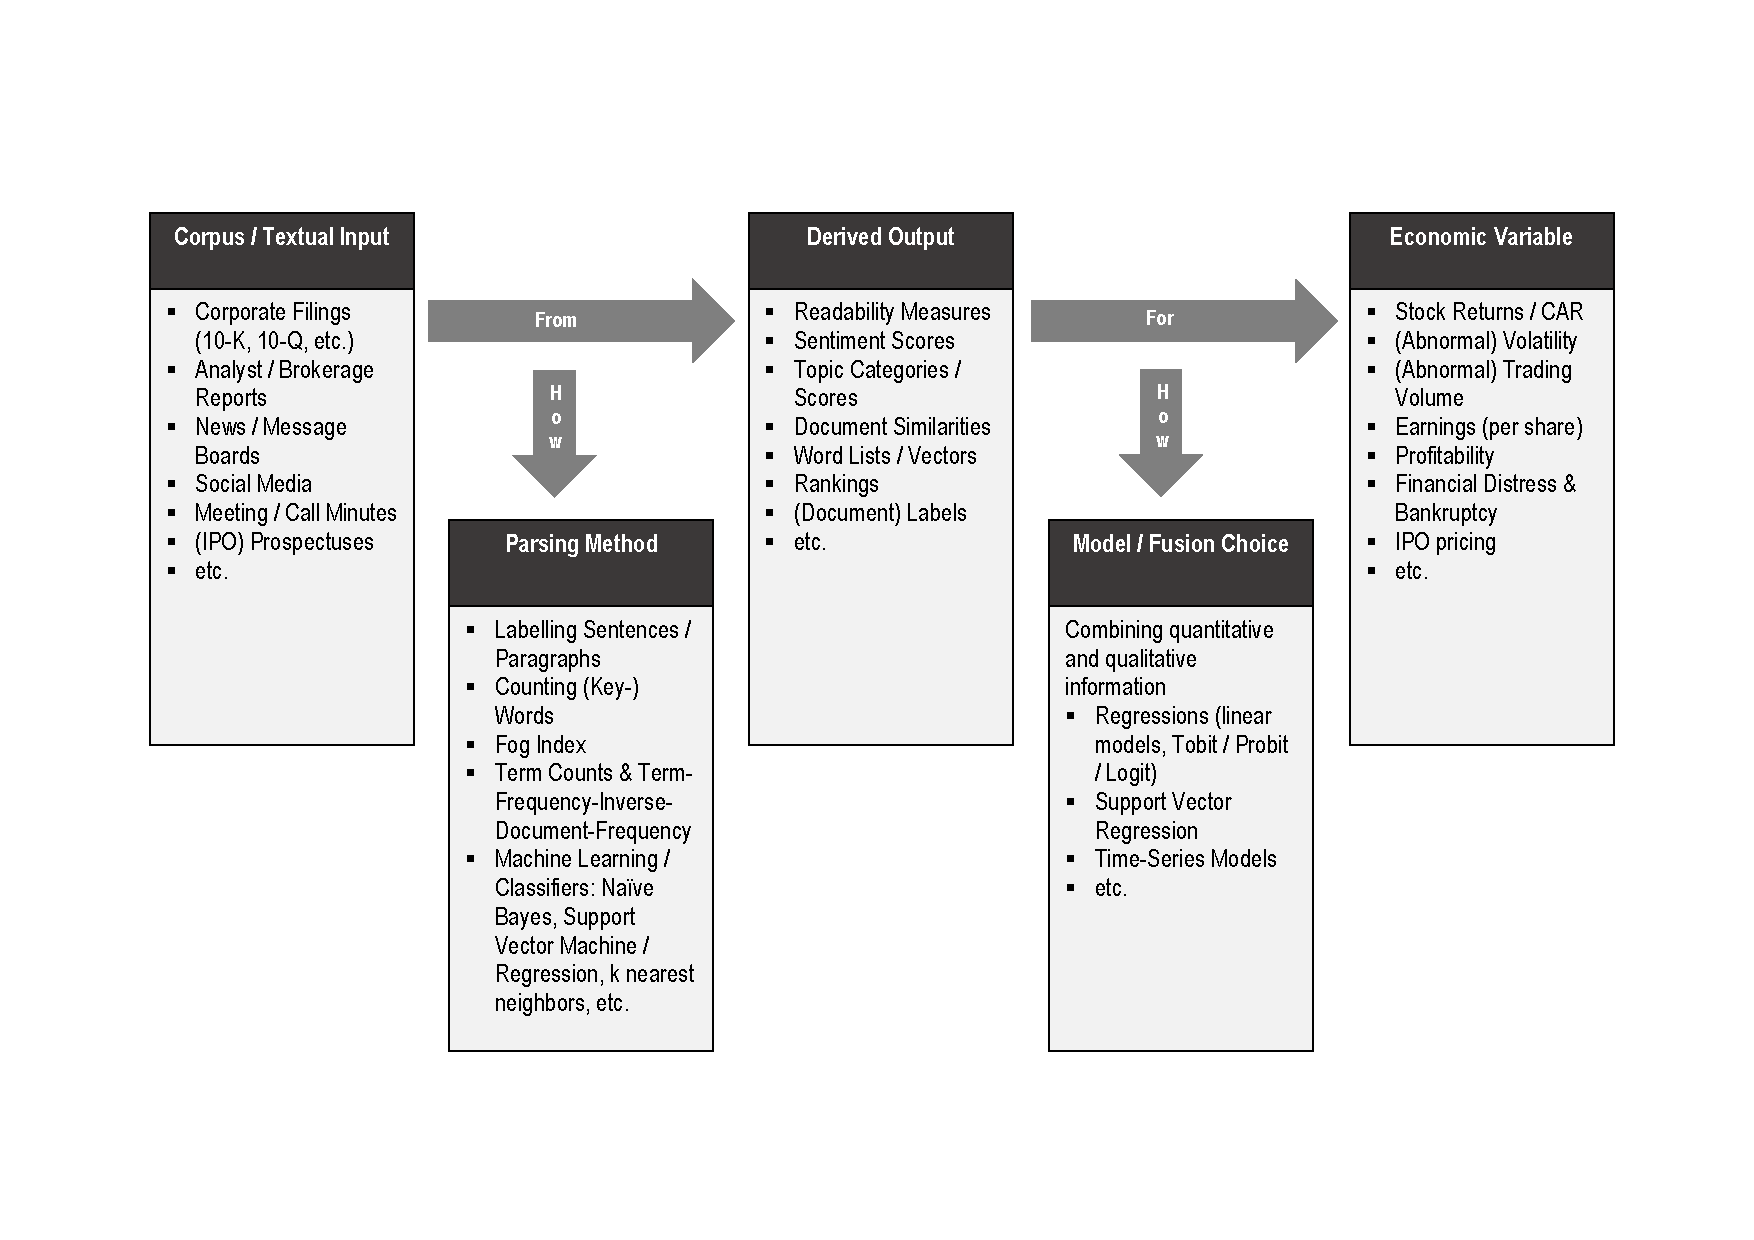
\includegraphics[width=\textwidth]{./Process_graph.pdf}
		\caption{Schematic Representation of a Research Process: Textual Analysis in Finance}
		%\source{Own Representation based on \textcite{LM-meta-2016, Das2014}}
		\label{fig: process_schema}
\end{figure}

In general, however, natural language processing in the financial domain comes with several obstacles and difficulties for the researcher. A fundamental question is related to an essential trade-off between signal and noise when choosing the research design; in other words, although analyses sometimes use simplifying assumptions\footnote{Most often this assumption reflects the idea that documents can be represented as so-called bags of words which allow the researcher to conduct an analysis on token-level, while at the same time this approach assumes that the ordering of words within a documents is irrelevant. I will further elaborate on this assumption in section \ref{ssec: senti_counts}, when I introduce the vector space model that will be the starting point for the analysis in this thesis.}, the attempt to better capture meaning and context also from a syntactic and semantic point of view can in some cases do more harm than good, because one simply adds more noise to the model that shall not be mistaken for signal \parencite{LM-meta-2016}. 

Further issues, which affect a lot of studies, are data availability, retrieval issues such as downloadability, document structure, and the subsequent parsing process. For some corpora, no collections or databases are available and require download by hand. Moreover, the downloaded files are often not available in the required format or are not machine-readable\footnote{In most cases, the property of being machine-readable is a minimum requirement for any corpus, so this is a rather theoretical side-note.}, or require at least a minimum amount of parsing. This imposes large practical problems, as \enquote{document parsing relies on consistency in the structure of the text and any related markup language} \parencite[1192]{LM-meta-2016}. This requirement is not always given in real-life applications, where data is often unstructured or inconsistent (over time)\footnote{I will further expand on one such issue when describing a corpus of 10-K* filings used in this thesis (see section \ref{sec: data_sample} about data collection and, specifically, footnote \ref{fn: parsing_LM})}. Other problems connected to the parsing procedure arise at the stage of tokenization or sentence-/paragraph-level segmentation. In this context, \textcite[1215]{LM-meta-2016} provide a good introductory overview of challenges and tripwires when applying natural language processing in the financial domain. In particular, the authors highlight issues which arise from what might sound like an obvious statement, namely that\enquote{all textual methods are based on first identifying words}. However, the undergoing of identifying \textit{words} is more subtle than it appears at first sight. One needs to clarify what happens, for instance, with compound words that are connected via hyphens (e.g., \textsf{well-known} or \textsf{up-to-date}), proper nouns (e.g., the \textsf{Fama} and \textsf{French} from the Fama-French-Model), and abbreviations (e.g., \textsf{FC} for football club or \textsf{Mr.} for Mister). Moreover, the example chosen for proper nouns reveals yet another problem: How can we deal with polysemy, i.e., the fact that the surname \textsf{French} (of famous economist Kenneth French) looks fully equivalent to the description of nationality (\enquote{to be of \textsf{French} origin/nationality}), yet the two words have very different meanings? This would require the researcher or the machine to learn from context, which in turn calls for usage of constructs that go above the granularity of a word-based analysis. For instance, this could be learned using n-grams (recognizing that the name \textsf{French} will likely tend to co-occur with words like \textsf{Mr.}, \textsf{Fama}, \textsf{Model}, etc.; whereas the nation-based version will rather co-occur with \textsf{British}, \textsf{German}, and so on). Furthermore, conjugations and declinations can impose problems: words like \textsf{calculate, calculates, calculated, calculating}, etc. all refer to the same word stem, yet are treated differently just because of their suffix. As I will describe in section \ref{ssec: senti_counts}, lemmatization and stemming deal with that exact problem -- in most cases by chopping off the endings and summing up those four instances as one single token (\textsf{calculat}). 

Similarly, also an apparently trivial task like splitting a document into sentences can prove to be tricky in practice. Generally, the parsing algorithm needs to be instructed on how to treat common sentence delimiters such as periods (\textsf{.}), colons (\textsf{;}), question marks (\textsf{?}), or exclamation marks (\textsf{!}). As \textcite[1216]{LM-meta-2016} evidence, the usage of \enquote{extensive lists, technical terminology, and other formatting complexities, makes sentence disambiguation especially challenging in accounting disclosures}. An illustrative example of this challenge would be the treatment of section headers such as \textsf{2.1. Financial Statements} or decimal separators as in \textsf{199.99 USD}. An inaccurate parser will -- based on the presence of the period sign -- mistakenly split the document at these points; and \enquote{the parsing errors in this case can be extraordinary}, implying that \enquote{Generic sentence parsing algorithms do not work well on financial documents} \parencite[1216, 1217]{LM-meta-2016}. This imprecision has crucial impact on the variable construction, implying the latter are therefore inherently measured with noise. For instance, most document readability measures, on which I will elaborate further in the next section, are constructed using the number of sentences in a document; and thus critically depend on how accurate we can identify sentences. 

\subsubsection{Readability}
\label{sssec: lit_rev_mining_readability}
Pioneering contributions in the stream of literature connected to readability of finance- and accounting corpora are \textcite{Li2008}, who evidenced that firms with lower current earnings (or earnings decreases) on average tend to produce less readable as well as longer 10-K filings\footnote{The argument provided suggests that management has an inclination to produce longer and more complex 10-K filings so as to diffuse or dilute bad news to investors. \textcite[221]{Li2008} labels this phenomenon \enquote{management obfuscation hypothesis}.}, and \textcite{DeFranco2015}. While the former \enquote{suggests a clear correlation between the linguistic features of annual reports and firm performance} \parencite[222]{Li2008}, the latter investigate the readability of security analysts' research reports. They find report readability to positively influence stock trading volume\footnote{A potential explanation for this reads as follows: if a report, ceteris paribus, classifies as \enquote{more readable}, the information conveyed in the document will be perceived as more precise information and thus trigger stronger trading signals for investors \parencite{DeFranco2015}.}, with the latter being a commonly used predictor for stock return volatility and thus relating to this thesis indirectly.

%\footnote{With reference to this notion, more readable research reports induce trading volume, which in turn is usually negatively correlated with return volatility. Hence, if the relationship between volume and volatility is safe to assume, more readable documents would correspond to lower volatility, which is in accordance to other findings (see \textcite{Loughran2014} as well as subsequent interpretations on \textcite{LehavyLiMerkley2011} in connection with \textcite{Schutte2007}).}. % CHECK FOOTNOTE AGAIN - SEE COMMENT BELOW

In a similar setting, \textcite{HsiehHuiZhang2016} relate stock price reactions to the degree of readability upon publication of analyst reports. They find that the cumulative abnormal return (CAR) in a $[-1,1]$-day window around the report issuance date increases by 58 basis points if the readability of the report increases by one standard deviation. A particularly important side note for this thesis is the statistical significance that \textcite{HsiehHuiZhang2016} as well as \textcite{DeFranco2015} find for one of their control variables, namely the narrative tone that analysts use -- thus indicating that not only readability but also textual sentiment matters for the market in determining price and volume for equity instruments\footnote{\textcite{DeFranco2015} additionally include an interaction term between readability and tone, which they find to be positive and significant. This suggests that these two variables reinforce each other.}.

% SHOULD INCLUDE THIS INTERACTOR AS WELL .....

\nomenclature{CAR}{Cumulative Abnormal Return}

In the area of volatility prediction based on readability of financial documents, the most relevant paper for this thesis is \textcite{Loughran2014}. They evidence that volatility, proxied by the post-publication-RMSE (from a market model), significantly decreases with the degree of readability of 10-K reports. Suggesting another, more indirect, channel of cause and effect in this context, \textcite{LehavyLiMerkley2011} have shown that less readable 10-K filings tend to be connected with increased analyst coverage\footnote{The authors provide a potential explanation for that phenomenon: a 10-K that is relatively difficult to read has too high processing costs for a single analyst to cover them. Thus, naturally, in order to meet investor's information demand, more analysts will start to track the stock and exert collective effort.}. Referring to the findings of \textcite{Schutte2007}, who evidence that analyst coverage initiation helps investors to better distinguish \enquote{true} firm-specific information from pure noise signals, this suggests that the fact that an analyst tracks the company \textit{per se} has a negative impact on firm-specific volatility. This interpretation undermines the findings of \textcite{Loughran2014}, namely that more readability in 10-K's (be it directly or via increased analyst coverage) reduces the stock price volatility of the companies submitting the filings.
\nomenclature{RMSE}{Root Mean Squared Error}

% THIS IS CONTRADICTORY: more readable means signal is clearer --> enhances trading volume and thus vola
% but LM 2014 state the opposite: "better written documents produce less ambiguity in valuation, as reflected by the lower price volatility of the stock in the period immediately following the filing"
% However, they acknowledge a potential alternative channel: "The positive relation between file size and volatility, earnings surprises, and analyst dispersion is inconsistent with the alternative explanation that file size is a proxy for disclosure (see Leuz and Schrand (2009)). If file size proxies for firm disclosure, one would expect larger documents to be negatively (not positively) related to volatility and analyst dispersion."

Regarding the \textbf{measurement} of readability, different metrics have evolved in the literature, with the most commonly used being the Gunning-Fog-Index as well as the Flesch-Kincaid-Grade-Level-Formula and the Flesch Reading-Ease Score (FRES)\footnote{All of these measures effectively are a linear combination of two components, namely the average length of sentences as well as proportion of \enquote{complex} words used, while complexity of words is determined by syllabication. A more detailed definition of these metrics is provided in appendix \ref{sec: annex_fogflesch}.}; nevertheless, \textcite[1649]{Loughran2014} argue that these measures, because they are too strongly focused on sentence length and word complexity, are not suitable in the context of business-related text. Moreover, they do not adequately account for differences in background knowledge between the targeted audiences. In fact, based on the Fog measure, very common words like \textsf{company}, \textsf{management}, or \textsf{financial} would be considered to be \enquote{complex} words -- yet they are still very likely to be understood by the average investor. Furthermore, all of the common readability measures require some form of parsing of the text and are thus exposed to typical inaccuracies and subjectivities connected to such procedures. In the work of \textcite{Loughran2014}, the \enquote{underlying} textual source were 10-K filings with the SEC. For these documents the authors suggest an alternative that is a much simpler, less error-prone and more reproducible metric, yet is still correlated to \enquote{conventional} measures like the Fog Index and equally able to capture readability: the natural logarithm of gross file size (measured in megabytes) of the 10-K filing\footnote{One should note at this stage that this approach requires the researcher to account for firm complexity (most likely using a proxy like firm size), as longer reports could be simply due to the complexity of the fundamental business \parencite{LM-meta-2016}. }.

\nomenclature{FRES}{Flesch Reading-Ease Score}

\subsubsection{Sentiment Analysis}
\label{sssec: lit_rev_mining_senti}

As \textcite{LM-meta-2016} indicate, the most simple approach to a textual analysis with financial corpora is to search the documents for appearance of certain keywords (or keyword phrases) of interest (for instance, they cite phrases like \textsf{ethic} or \textsf{corporate social responsibility}, whose frequency can be used when one attempts to quantify corporate governance metrics or the probability of lawsuits). A natural extension of this methodology involves to not look for specific phrases only, but rather use a dictionary of words\footnote{Throughout this thesis I will use the words lexicon, dictionary, or (sentiment) word list interchangeably; although from a linguistic and literary point of view they are not equivalent.}, all of which carry a similar characteristics. In the large majority of cases these word lists are chosen so as to share common sentiment and thus relate directly to the technique of sentiment analysis. 

The frequency of sentiment words is then often aggregated into a scalar, constructing what is often referred to as \enquote{sentiment index} or \enquote{sentiment score}\footnote{Note that the strong focus on keyword counting in sentiment analysis has lead the discipline to be dominated by vector space models (or, equivalently, term-document-matrices) within the bag-of-words framework (see section \ref{ssec: senti_counts} where I will elaborate on these concepts for the sake of introducing the research design applied in this thesis.}. Apart from the usability as a variable in many research applications, sentiment indices are common also in practice, as the following quote undermines:
\blockquote[\textcite{McKinsey_2013}]{Gauging sentiment with an index makes it possible for machines to analyse the information; it can be converted, aggregated, and compared. And the index can be used with statistical analysis to build prediction models. Obviously, the difficulties come in the details of assigning the sentiment index. At the core of the process is a lexicon that lists words or phrases that represent a certain kind of sentiment and, importantly, reflect the specific context in which the text appears.}

The last part of the definition highlights a critical fact or that distinguishes sentiment analysis in finance and accounting from other disciplines: while early studies used \enquote{generic} lexica\footnote{The most prominent choice for word classification among the heap of lexica available was the Harvard General Inquirer (GI) (in particular, the Harvard IV-4 dictionary, see \url{http://www.wjh.harvard.edu/~inquirer/homecat.htm}).} that were developed from and thus suitable for texts in psychology and sociology, \textcite{Loughran2011} were the first to recognize that those lists are not applicable to documents in the business domain. In fact, using 10-K filings, the authors find that almost three quarters of allegedly negative words in the Harvard IV-4 list do not appear to be negative in business context\footnote{For instance, such words are \textsf{tax, cost, capital, board, liability, foreign}, and \textsf{vice}, which appear very often in 10-K filings, yet are very likely not negatively connoted \parencite[36]{Loughran2011}.}. Therefore, \textcite{Loughran2011} created finance-specific sentiment word lists in the following categories: Negative, Positive, Uncertainty, Constraining, Litigious, Strong/Modest/Weak Modal. These lists (especially the negative lexicon) have become the \enquote{gold standard} in financial sentiment analysis and are also the backbone of this thesis. Henceforth, I will label these word lists using the acronym LM dictionary (or lexicon/word list). 

\nomenclature{LM (Dictionaries)}{Sentiment Dictionaries developed in \textcite{Loughran2011}}

Turning from this methodological introduction to relevant literature contributions, a good starting point for dictionary-based sentiment extraction is the paper of \textcite{YukselturkTucker2015}. They calculate thematic net sentiment scores for a UK-based sample of analyst research reports by classifying (80 to 180) keywords contained in six theme-buckets\footnote{The six themes are the following: macroeconomic and regulatory environment, industry and market environment, growth, management and strategy, financial performance, financial position.} into positive and negative keywords, while the classification task was performed using both Harvard IV-4 and LM dictionaries. The main finding was that theme-related (net) sentiment affects the two key outputs (recommendations and target prices) of the research analyst. \textcite{HuangZangZheng14} extended this stream of research regarding textual contents of analyst reports. They quantified sentiment of sentences contained in analyst reports using a Naive Bayes machine-learning algorithm. After controlling for a simultaneous change in the quantitative summary metrics (i.e., price target, stock recommendation and EPS forecast), they show that the textual opinion embedded in the respective analyst report helps to explain abnormal stock returns subsequent to the release of the report. Moreover, they evidence that the narrative content of analyst reports also carries \enquote {predictive value for future earnings growth in the subsequent five years} \parencite[2151]{HuangZangZheng14}. 

In the same category of research falls also an important paper of \textcite{Tetlock2007}. He mined a popular column in the \textit{Wall Street Journal} in order to gauge market sentiment; in particular, he constructed a pessimism index using the Harvard GI lexicon, which was shown to be predictive for lower subsequent returns and higher volatility.

Another pioneering paper in this area of research, which due to its nexus to volatility prediction is also relevant for this work, is \textcite{AntweilerFrank2004}. They analysed more than 1.5 million messages from message boards about 45 companies; using the Naive Bayes approach to classify messages to either buy, hold, or sell category. The single classified messages were then aggregated into a bullishness as well as an agreement index, which proved to be successful in predicting trading volume as well as volatility, but unsuccessful in explaining stock returns. Regarding volatility, only the bullishness seems to carry explanatory power while the the correlation is positive (i.e., more bullish messages today imply greater volatility tomorrow); agreement between message posters does not help to predict realized volatility. 

Most importantly, however, this thesis builds upon the work in \textcite{Kogan2009_1}, which was extended in \textcite{TsaiWang2012, TsaiWang2013, TsaiWang2014, TsaiWangChien2016, WangTsaiLiuChang2013} and more importantly in \textcite{TsaiWang2016}; all of which essentially show that textual sentiment of 10-K's helps to explain stock return volatility in the quarter/year after the filing (either in a ranking or regression framework). These results were yet further refined in \textcite{Rekabsaz2017}, who used a more elaborate word weighting scheme on the LM sentiment lists and furthermore investigated on potential industry-specific patterns. 

\subsubsection{Text Analysis Using 10-K Filings Corpora}
\label{sssec: lit_rev_mining_10K}

As is evident from the literature review up to this point, corporate filings as a mandatorily disclosed document provide a rich source of potential research questions in the textual analytics field and are very popular within the finance and accounting domain. In this context, \textcite[223]{Das2014} points out\footnote{In that regard, \textcite[3]{KearneyLiu2014} highlight that while corporate disclosures provide \enquote{a natural source of textual sentiment for researchers insofar as they are official releases}, their main disadvantage \enquote{is the low frequency of the data, because firms usually make these disclosures on a quarterly or annual basis.}}: 
\blockquote{Whereas much of financial text analysis uses messages posted to finance boards like Yahoo!, Motley Fool, or to blogs such as Twitter, Facebook, etc., other textual analysis has been applied to company reports and filings. In the former case, analysis is usually of a time series nature, whereas in the latter, text analysis is undertaken across companies in a cross-section.}

Regarding the heap of corporate filings available, \textcite[227]{Das2014} further highlights that most of the literature is focussing on 10-K filings because these are considered to be the most informative document for (potential) investors\footnote{I follow this stream of literature and use a broad corpus of 10-K*'s (refer to footnote \ref{fn: 10K-def} for a description of variants of the \enquote{standard} 10-K). Moreover, to avoid permanent repetition I will use the terms 10-K, filing, or annual report synonymously, although the \textcite{SEC} highlights that \enquote{10-K typically includes more detailed information than the annual report to shareholders.}}. 10-K reports are mandatory disclosure documents that are to be filed annually with the SEC. As it is pointed out on their web-page\footnote{See \url{https://www.sec.gov/fast-answers/answersreada10khtm.html}, accessed on 07/31/2018.}, the report's contents contain an important source of information and decision-making material for investors: \enquote{Among other things, the 10-K offers a detailed picture of a company's business, the risks it faces, and the operating and financial results for the fiscal year. Company management also discusses its perspective on the business results and what is driving them.} As \textcite{Pulliza2015} points out and what is of direct importance for all language analytics studies using this corpus, 10-K filings shall be conform with the SEC Plain English Rule, which was established with the target that communication from the management towards the investor community is written in plain and understandable terms without an overload of complexity.

One should note that this part of the literature review reflects only \enquote{related} contributions, i.e., publications with a focus on natural language processing and, more specifically, sentiment analysis. The (much broader) stream of literature that deals with the \enquote{quantitative} outputs of (mandatory) corporate disclosure and the information content as well as the market reactions of such disclosures, is not part of this review. This, for instance, encompasses a large range of publications in the field of accounting policies (accounting standards, international comparisons, etc.) and manipulation methods (with contributions related to (abnormal) accruals mainly) as well as mergers and acquisitions including the subsequent purchase price allocations (with contributions related to intangible assets, goodwill, etc.) that are disclosed in annual filings. In fact, I view the combination of such \enquote{hard} information content with the textual tone as a much desired extension for further research; a fact on which I will further elaborate in the conclusions of this thesis (cf. section \ref{sec: conclusion}). 

One of the first questions to ask when analysing 10-K filings is whether to text mine the whole document or rather target a specific section in it. The most famous of them, which is often said to be the most informative and carry the most forward-looking statements, is Item 7 of the 10-K filing, which is referred to as \textit{Management Discussion and Analysis} (MD\&A). For instance, this section is the subject of study in widely cited papers like \textcite{Kogan2009_1, Li2010, Feldman_et_al_2010, TsaiWang2012, WangTsaiLiuChang2013, TsaiWang2013, TsaiWangChien2016, TsaiWang2016}. 

Another common choice is \textit{Item 1A - Risk Factors}, \enquote{which contains information about the most significant risks for the company} \parencite[1712]{Rekabsaz2017}, which is used, among others, in \textcite{HuangLi2011} and \textcite{Rekabsaz2017}. A good overview of all sections within a 10-K filing is provided on the SEC web-page\footnote{See \url{https://www.sec.gov/fast-answers/answersreada10khtm.html}, accessed on 7/31/2018}.  

However, also section-based analysis comes with obstacles: As \textcite{LM-meta-2016} point out, parsing algorithms struggle with the fact that some 10-K submissions are unstructured (especially before 2002), some sections are mislabelled (e.g., MD\&A is falsely tagged as Item 6 instead of 7), or that companies place content across different parts of the document and cross-reference across the filing using footnotes. Regarding the latter, \textcite{HeidariFelden_Footnotes_2015} presented a promising idea, that might be an interesting extension to 10-K corpus based research: they tried to categorize income tax footnotes within 10-K and 10-Q's into pre-defined buckets and proved that machine-based classifiers can achieve the same task with relatively high accuracy, allowing the researcher to extract content from an \enquote{unstructured} part of the filing without the necessity of reading the footnotes manually. This was extended upon by \textcite{Amel-Zadeh_Faasse_2016} and \textcite{ThinggaardJeppersenMadsen2016}, who compared MD\&A content with footnote disclosure, the latter doing so for the Danish market and therefore belonging to the absolute minority of publications which use non-US based data.

The most influential papers who focus on the 10-K as single, homogeneous document are \textcite{KothariLiShort_2009, LehavyLiMerkley2011, Loughran2011, Loughran2014, LM-meta-2016}, while good introductory overviews about 10-K language processing (and, more generally, textual analysis in finance and accounting) are provided by \textcite{Qiu07, Pulliza2015, LM-meta-2016}. 

\nomenclature{MD\&A}{Management Discussion and Analysis (Section within a 10-K Filing)}

\subsubsection{Commoly Used Techniques and Algorithms}
\label{sssec: lit_rev_mining_algos}

I will briefly present a few common methodologies and algorithms, which are used particularly often in text classification\footnote{Text classification can be described as the mining of text for certain features, and then, based on those features, assign to the document a label, which comes from a fixed set of pre-defined, discrete values.} problems and therefore are commonly applied in sentiment analysis as well. All of the presented algorithms fall under the category of \textbf{supervised} machine learning. A recommendable study that offers further (and more detailed) insights into most frequently applied machine-based techniques is provided in \textcite{GuoShiTu2017}. 

\begin{enumerate}[(1)]
\item \textbf{Naive Bayes.} The Naive Bayes algorithm is \enquote{one of the oldest, most established methodologies to analyze text} \parencite[1209]{LM-meta-2016}. It allows the researcher to classify a large amount of data for a fairly small yet most often hand-classified training subset and is also able to handle multi-label classification (i.e., classifiers with more than binary label realizations). \textcite{HuangZangZheng14} define the Naive Bayes classification algorithm as follows:
\blockquote{The Naive Bayes classification is a statistical learning method that assigns the textual document to the most likely category based on the statistical relation between words and categories learned from a training dataset. \textelp{} The Naive Bayes classification can be viewed as a prediction model, with the words in the document as the input variables and the probability of the opinion categories as the predicted value.}

Thus, in the case of Naive Bayes, the task is to assign to each document $d$ a certain class $c$ out of $L$ possible choices, i.e., $c \in \mathcal{C} = \{c_1, c_2, \dots, c_L \}$. For instance, classes can be binary  $\{\text{positive}, \text{negative} \}$ or multi-categorical (such as $\{\text{good}, \text{bad}, \text{neutral} \}$). The way this is achieved is by choosing the appropriate class $c$ which maximizes the conditional probability $P[c|d]$. Using Bayes Rule and dropping the denominator (which serves as \enquote{scaling} constant and does not vary with respect to the class assigned), this corresponds to $P[d|c] P[c]$. Representing document $d$ as a bag of the $J$ words $v_1$, $v_2$, $\dots$, $v_J$ in it, this conditional probability can be written as $P[v_1, v_2, \dots, v_J|c] P[c]$. The key assumption of the algorithm regards the first term, and also explains why the method is called \enquote{naive}: one simply assumes that the conditional probabilities $P[v_j|c], j = 1, \dots, J$ are independent from each other; thus simplifying the maximization task to $ P[c] \prod_{j=1}^{J} P[v_j|c] $. All those probabilities can be estimated as simple fractions from the training sample \parencite{Jurafsky_Draft_2017}. 

The Naive Bayes algorithm has proven his success in classification tasks in different publications and across different \enquote{underlying} textual bases. For instance, \textcite{Li2010} used the method to classify the managerial opinion section in financial statements, while \textcite{AntweilerFrank2004} were the first to apply it in order to track investor sentiments in Internet stock message boards. As already mentioned, \textcite{HuangZangZheng14} used Naive Bayes it to categorize more than 27 million sentences in analyst reports. The most important \textit{practical} application of the Naive Bayes algorithm is spam-detection/filtering \parencite{Jurafsky_Draft_2017}. 

As \textcite{Zhang04} points out, the Naive Bayes algorithm performs surprisingly well in real-world classification tasks, although the conditional independence assumption is hardly ever met in practice. One \enquote{basic} explanation is that one actually does not care about the accuracy of probability estimation for as long the assigned maximum probability and thus category is correct. For instance, the true probability of observing a positive sentence (or paragraph, or even whole document, as is the case, for instance, for tweets or shorter messages) given a set of words (features/attributes) in a document might be 90 percent; implying that the probability of observing a negative class is ten percent. If the Naive Bayes algorithm predicts the probabilities to be 55 percent and 45 percent, respectively, the estimation accuracy itself is rather poor – whereas the classification task is nevertheless performed correctly (because $.55 > .45$, as is the case for $.9 > .1$). In other words, Naive Bayes might produce a bad estimate for the class probabilities, but this may not too dramatic in real world tasks as the classification is considered correct so long as the correct class is simply more probable than the wrong one\footnote{\textcite{Zhang04} adds to the explanation of \textcite{Domingos1997} and asks the question why an existing dependence between attributes might not \enquote{flip the classification}, i.e., make probability estimates such as 39 percent (positive class) versus 61 percent (negative class) in our above example. He theoretically proves that Naive Bayes is an optimal classifier, if either the dependencies among attributes support the same classification or, in the case of supporting a contrary classification, they \enquote{cancel each other out}. This is the case if both the local and global distribution of dependencies satisfy appropriate conditions.}. 

With respect to the dictionary-based method applied in this thesis, \textcite{GuoShiTu2017} indicate that the machine-based Naive Bayes learner does not necessarily outperform lexicon methods, as the usage of the full training set can introduce noise into the classification process compared to pre-selected lexicon words. Conflicting with this view, \textcite{HuangZangZheng14} find that Naive Bayes beats dictionary approaches in terms of classification accuracy on a sample of sentences contained in analyst research reports. 

\item \textbf{Support Vector Machines.} The Support Vector Methodology can be used either as classifier (often associated with the terminology of Support Vector \textit{Machine}, SVM) for discrete label prediction or also in a regression framework (accordingly named Support Vector \textit{Regression}, SVR) for continuous output variables. A good introduction of the algorithm is provided in \textcite{ManningSchutze_IR_2008, GuoShiTu2017, Rekabsaz2017, GavrishchakaBanerjee2006}.

In short, the classification problem can be formulated as follows\footnote{The large part of the following derivation is from the machine learning MOOC from Professor Yaser Abu-Mostafa (California Institute of Technology), available at \url{http://work.caltech.edu/lecture.html} as well as The MathWorks, Inc. (\url{https://www.mathworks.com/help/stats/support-vector-machines-for-binary-classification.html} and \url{https://www.mathworks.com/help/stats/understanding-support-vector-machine-regression.html}, respectively). All three URLs were accessed on 08/01/2018.}: One starts with a set of $P$ training data pairs $(\mathbf{x_i}, y_i)$, $i = 1, 2, \dots, P$ where $\mathbf{x_i} \in \mathbb{R}^L$ is a $L$-dimensional input (feature) vector, and $y_i \in \{y_1, y_2, \dots, y_P \}$ is a scalar, which defines the corresponding label for feature vector $\mathbf{x_i}$. 

In a graphical (two-dimensional) manner, the support vector classifier seeks to find a hyperplane $\mathbf{w^T} \cdot \mathbf{x} - b$ with $\mathbf{w} \in \mathbb{R}^L$ and $b \in \mathbb{R}$, so that this very hyperplane places each pair $(\mathbf{x_i}, y_i)$ on the \enquote{correct side} of the hyperplane. Under the assumption that the label is binary, i.e., $y \in \{ -1, +1\}$ this means that positively labelled pairs should be on one side of the hyperplane, while negatively labelled pairs should be on the other side. Mathematically, this means that all points need to satisfy the following constraint: $\forall i: y_i (\mathbf{w^T} \cdot \mathbf{x_i}) - b \geq 1$ 

While there are many such hyperplanes, SVM seeks to maximize the distance between those $\mathbf{x_i}$'s, which lie closest to the hyperplane. In other words, when trying to find the label for a \enquote{newly observed} vector of features $\mathbf{x_i}$, one tries to minimize the possibility of making a classification error. Geometrically, this achieved by maximizing the \textit{distance} between so-called \textbf{support vectors}. We call support vectors all those $\mathbf{x_i}$'s which lie \enquote{exactly on the margin}, i.e., satisfy the constraint $y_i (\mathbf{w^T} \cdot \mathbf{x_i}) - b = 1$ with \textit{equality}. Given that the distance between support vectors can be expressed as $\dfrac{2}{\lVert \mathbf{w} \rVert}$, the maximization can reversely be formulated as:
\begin{align*}
\underset{\mathbf{w} \in \mathbb{R}^L}{\text{min.}} \quad & \dfrac{1}{2} \mathbf{w^T} \cdot \mathbf{w} \\
\text{s.t.} \quad & \forall i: y_i (\mathbf{w^T} \cdot \mathbf{x_i}) - b \geq 1
\end{align*}
Applying the Lagrangian method with $P$ multipliers $\alpha_i$, $i=1, 2, \dots, P$, one can use Karush-Kuhn-Tucker (KKT) first-order conditions (FOC) of the \textit{primal} to formulate the \textit{dual} as follows:
\begin{align*}
\underset{\mathbf{\alpha} \in \mathbb{R}}{\text{min.}} \quad &  \dfrac{1}{2} \sum_{i=1}^{P} \sum_{j=1}^{P} y_i y_j \alpha_i \alpha_j \highlight{\mathbf{x_i^T} \cdot \mathbf{x_j}}  - \sum_{i=1}^{P} \alpha_i \numberthis \label{eq: SVM} \\
\text{s.t.} \quad & \forall i: \alpha_i \geq 0 , \sum_{i=1}^{P} \alpha_i y_i = 0
\end{align*}
Obtaining solutions for the Lagrange multipliers $\alpha_i$ using quadratic programming\footnote{Note that most of the $\alpha_i$'s will be zero, as they are strictly positive only for the support vectors of the problem. The KKT condition reads $\alpha_i [ y_i (\mathbf{w^T} \cdot \mathbf{x_i}) - b) - 1 ] = 0 $, implying that for many vectors the term within squared brackets will be positive and the multiplier will guarantee the whole expression to be zero; for support vectors, however, the part within squared brackets is zero by definition, thus \enquote{allowing} the $\alpha_i$'s to be positive.}, we can find the weight vector that solves the problem by using the FOC of the primal, i.e., $ \mathbf{w} = \sum_{i=1}^{P} \alpha_i y_i \mathbf{x_i}$. Note that this is a $L$-dimensional vector, as is the input vector $\mathbf{x_i} \in \mathbb{R}^L$. Similarly, the last remaining term that defines the optimal separating hyperplane, $b$ (often called \enquote{bias} term), can be found using any of the support vectors (say support vector $\mathbf{x_m}$), and solving $y_m (\mathbf{w^T} \cdot \mathbf{x_m}) - b = 1$. 

One key advantage of the SVM is the avoidance of in-sample overfitting, as the classifier is defined only by the support vectors, discounting the impact of noisy features. Secondly, and partly related to the first advantage, SVM -- due to its dependence on dot products -- allows the usage of the so-called Kernel trick for \textit{non-linear} classification tasks \parencite{GuoShiTu2017}\footnote{The second methodology to handle data that is not linearly separable, is to \enquote{allow for errors}, i.e., violations of the margin, in a so-called \textbf{soft-margin SVM}. In other words, most often one does not require the algorithm to satisfy classification with a strict accuracy of one hundred percent. Denoting with $\xi_i \geq 0$ the slack around vector $\mathbf{x_i}$ and introducing a regularization constant $C$ that dictates how heavy one penalizes the sum of classification errors, we can write:
\begin{align*}
\underset{\mathbf{w} \in \mathbb{R}^L}{\text{min.}} \quad & \dfrac{1}{2} \mathbf{w^T} \cdot \mathbf{w} + \dfrac{C}{P}  \sum_{i=1}^P \xi_i \\
\text{s.t.} \quad & \forall i: y_i (\mathbf{w^T} \cdot \mathbf{x_i}) - b \geq 1 - \xi_i
\end{align*}
The dual formulation reads exactly the same as in the hard-margin SVM, with the only exception being the constraint on the Lagrange multipliers, which in this case are not only non-negative, but also smaller than $C$, $\forall i: 0 \leq \alpha_i \leq C$. In practice, both soft-margin and kernel trick are often used together.}. 

The key of the Kernel transformation lies in the observation that the number of solution parameters $\alpha_i$ depends solely on the number of training data available, i.e., it is always $P$ and does not depend on the dimensionality of the feature space (which we assumed to be $\mathbb{R}^L$ so far)\footnote{This can be seen by observing the gray-shadowed term in equation \eqref{eq: SVM}, namely $ \mathbf{x_i^T} \cdot \mathbf{x_j} $. This is a \textbf{dot product} of two $L$-dimensional vectors, returning a scalar. Equivalently, so does the dot product of two $Z$-dimensional vectors, thus leaving the complexity of the optimization task unaltered.}. Thus, the difficulty of solving the problem is equivalent, even if one moves into a higher-dimensional space $\mathbb{R}^Z$ with $Z>L$, while at the same time one might obtain linear separability in $\mathbb{R}^Z$. 

What is referred to as Kernel \textbf{trick} corresponds to the following idea: given two feature vectors $\mathbf{x_i}$ and $\mathbf{x_j}$, one can define the function $\mathbf{z_i^T} \cdot \mathbf{z_j} = K(\mathbf{x_i}, \mathbf{x_j})$, where $K(.,.)$ is called the kernel. Then, the highlighted part in equation \eqref{eq: SVM} can be rewritten as $\mathbf{z_i^T} \cdot \mathbf{z_j}$, thinking of $\mathbf{z_k}$ as a \enquote{transformation} of $\mathbf{x_k}$, leaving everything else unchanged and instead finding the optimal hyperplane in $\mathbb{R}^Z$. As one can see, the requirement for $K(.,.)$ is to return the dot product in $\mathbb{R}^Z$\footnote{Technically, for a function $K(.,.)$ to qualify as a kernel, we require that it is symmetric, and, in addition, fulfils so-called Mercer's condition.}. The \enquote{trick} lies therein that one can use \enquote{pre-defined}, i.e., \textbf{given}, kernels $K(.,.)$, which can be shown to guarantee the existence of the dot product $\mathbf{z_i^T} \cdot \mathbf{z_j}$. The most popular functions are the linear kernel, polynomial kernel, Gaussian kernel (often called Radial-Basis Function, RBF), and sigmoid kernel. 

For illustrative purposes, this introduction covers only the SVM for binary classification purposes; several extensions to this basic model have been proposed (such as SVM for multi-label classification, SVM for ranking purposes, and SVR for labels in a  continuous design, see \textcite{ManningSchutze_IR_2008}). Due to its broad applicability as well as good results (especially in the classification framework), SVM has been applied extensively in the literature. The most relevant academic contributions in the field of text analysis in finance and accounting for this thesis are \textcite{Kogan2009_1, TsaiWang2012, TsaiWang2013, WangTsaiLiuChang2013, TsaiWang2014, TsaiWang2016, TsaiWangChien2016, Rekabsaz2017}.

\nomenclature{SVM}{Support Vector Machine}
\nomenclature{SVR}{Support Vector Regression}
\nomenclature{FOC}{First Order Condition(s) (of an Optimization Problem)}
\nomenclature{KKT}{Karush-Kuhn-Tucker (Condition(s) of an Optimization Problem)}
\nomenclature{RBF}{Radial Basis Function}

\item \textbf{Other.} Other well-studied text classification algorithms include, among others, the (multinomial) Logistic Regression (also called Maximum Entropy), k-Nearest Neighbour (k-NN), Latent Semantic Analysis, Latent Dirichlet Allocation, and Neural Networks \parencite{Jurafsky_Draft_2017}; however, to date hey are less commonly applied in textual processing in the finance and accounting domain.

\end{enumerate}

ad NB: Include why I can not use it here on doc-level (sentence level would be feasible).

\clearpage